\chapter{cute 之 Layout}

\begin{center}\small 作者：reed（知乎 @reed-84-49，专栏「CUDA高性能编程」）\quad 原文：\url{https://zhuanlan.zhihu.com/p/661182311}\end{center}

计算机中的内存是一维的线性地址空间，而数学计算问题所要处理的空间经常是高维的。如GEMM（General Matrix Multiplication）问题的数学计算体系是二维计算空间，Deep Learning计算体系是三维以上的计算空间(batch, height, width, channel, etc.)。如何高效的表达高维计算空间，如何高效便捷的将计算所要求的高维空间映射到一维空间变得越来越重要。

历史上对该问题的探究可以分为三个阶段：

\begin{itemize}
  \item 第一阶段BLAS的row/col-major + leading dimension描述阶段；
  \item 第二阶段Tensor的shape + stride阶段；
  \item 第三阶段为Hierarchy Tensor阶段。
\end{itemize}

二十世纪七八十年代开发的BLAS（Basic Linear Algebra Subprograms）库中描述矩阵时面对的问题多为二维问题，其通过引入行优先、列优先的概念来刻画一维存储结构和二维逻辑结构的映射关系。为了做某个维度的地址对齐、padding等，引入了leading dimension的概念，其可以描述第二个维度上数据的连续性关系。二十一世纪初Deep Learning在模式识别等领域暂露头角，各种框架应运而生，在Deep Learning计算中为了提升计算密度batch化成了重要手段，这时高维数据的描述成为必须，相关人员在blas中leading dimension基础上进行了扩展，引入了shape和stride描述体系。shape stride描述体系可以很好的刻画一维存储结构和高维逻辑结构的映射关系，并且使得某些操作只需要改变shape stride描述无需对数据实体进行移动，在stride的帮助下通过简单的coordinate和stride点积既可以完成逻辑地址和一维索引的映射。shape stride描述可以表达简单的高维数据，但是其对于具体的维度的轴必须是单调的，在数据的连续性方面要求比较严格。2023年层级的Tensor（Hierarchy Tensor）描述被提出，其在shape stride描述的基础上添加了具体的轴的层级描述（Graphene Tensor IR）[1]，使得数据在某个具体的轴上可以有更为丰富的表达。对于现代GPU计算体系而言，Tensor的分块和复杂映射都可以通过该层级体系（描述+代数）来表达和推导，其构建了复杂逻辑空间和硬件排列映射的一条途径。

Tensor的层次化描述体系在Graphene Tensor IR中进行了详细的描述；在具体实现方面，NVidia开源的cutlass模板中也利用同样的思路进行Tensor描述和计算。为了更好的抽象和利用编译时优化，cutlass利用了C++17实现了cute，它定义了层次化Tensor体系和其之上的代数计算，然后基于该cute描述体系实现了最新hopper架构之上的矩阵运算。Tensor是数据的表达，其表达一个相对独立且有结构的数据体，而Tensor内的数据排布则由Layout来表达。本文将关注这种映射结构，即Layout。本文在行文组织结构上：首先以示例的形式介绍一维向量的表示、二维矩阵的表示，然后介绍层次化的Tensor表示，再后介绍cute中常用的编译时和运行时形状描述，最后本文总结Layout的功能。

简单地讲，引入有层次的描述（Layout）代数来表达计算空间和一维地址空间的映射问题。Layout 是一个数据排列的描述体系，其可以实现将逻辑坐标映射到索引坐标（offset表示）。Layout包含Shape和Stride两部分。其中Shape描述排列的分块层次和结构。Stride描述块内或块间的数据排列连续性。Shape和Stride都是层级的嵌套表示。也就是说Shape可以包含Int数据和Shape。Shape和Stride需要有相同的层次关系。

在介绍有层次的Layout之前，我们先回顾无层次的Layout描述，也就是shape和stride描述的高维tensor。

\section{一维向量的表示}

Shape: (8), Stride: (1) 表示该排列包含8个逻辑位置，在逻辑位置和物理（数据）做映射的时候每一个元素之间的差为1，如图1所示其描述了0-7总计8个数字，其计算逻辑为 index\_physical = index\_logical * stride;

\begin{figure}[htbp]\centering
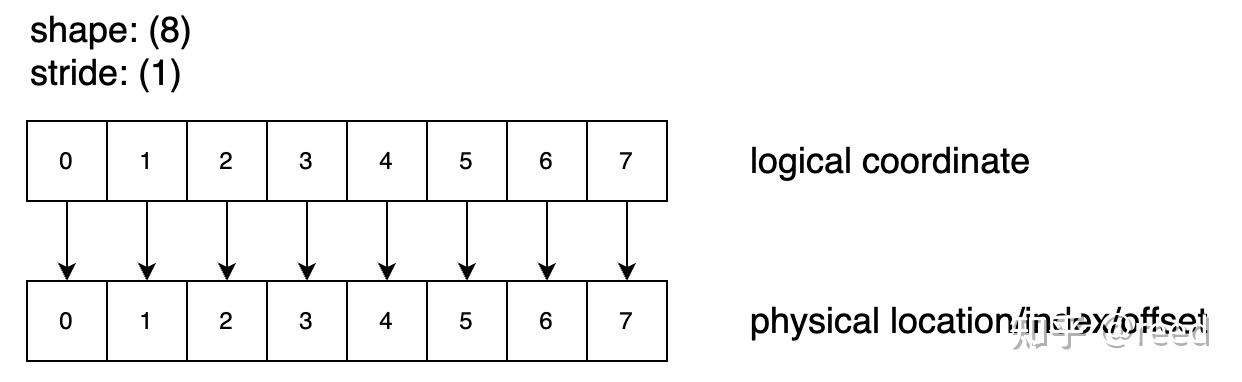
\includegraphics[width=0.9\textwidth]{figures/reed-01-layout/fig-01.jpg}
\end{figure}

Figure 1. shape = 8, stride = 1的逻辑空间和物理空间映射关系

Shape: (8), Stride: (2)表示该排列包含8个逻辑位置，每一个位置的坐标为自然序列0-7，如图2所示，其对应物理位置映射时的公式为 index\_physical = index\_logical * stride; 这时候我们发现逻辑空间和物理空间的大小是不一样的，在cute体系下，逻辑空间可以被称作domain，而代表存储的物理空间称作codomain，也就是size(tensor) = 8, cosize(tensor) = 15.

\begin{figure}[htbp]\centering
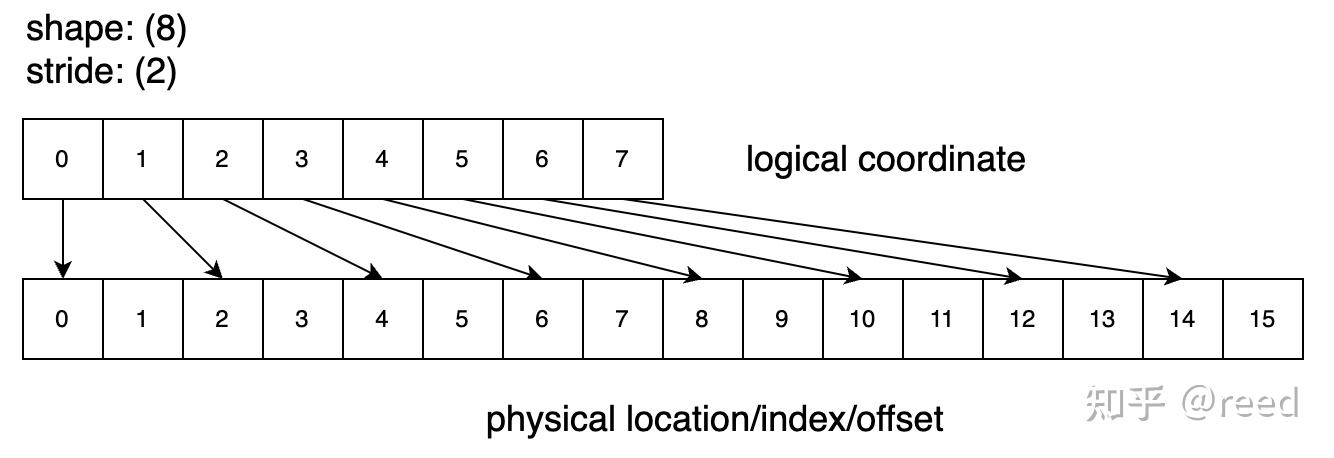
\includegraphics[width=0.9\textwidth]{figures/reed-01-layout/fig-02.jpg}
\end{figure}

Figure 2. shape = 8，stride = 2的逻辑空间和物理空间的映射关系

Shape: (8), Stride: (0)表示逻辑上我们需要的8个数据都来自于同一个存储位置0，如图3所示，所有的元素都指向同一个物理位置，通过图示也可以看到该layout的cosize为1。

\begin{figure}[htbp]\centering
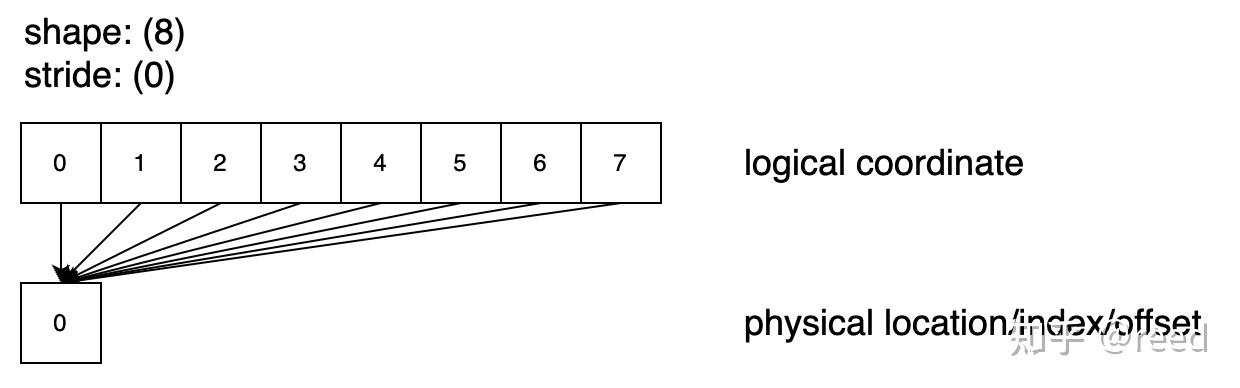
\includegraphics[width=0.9\textwidth]{figures/reed-01-layout/fig-03.jpg}
\end{figure}

Figure 3. shape = 8, stride =0的逻辑空间和物理空间的映射关系

Shape: (8), Stride: (-1) 通过Stride设置为-1可以实现对数据的前向访问，并且顺序是reverse的，这种case很少用到。

\begin{figure}[htbp]\centering
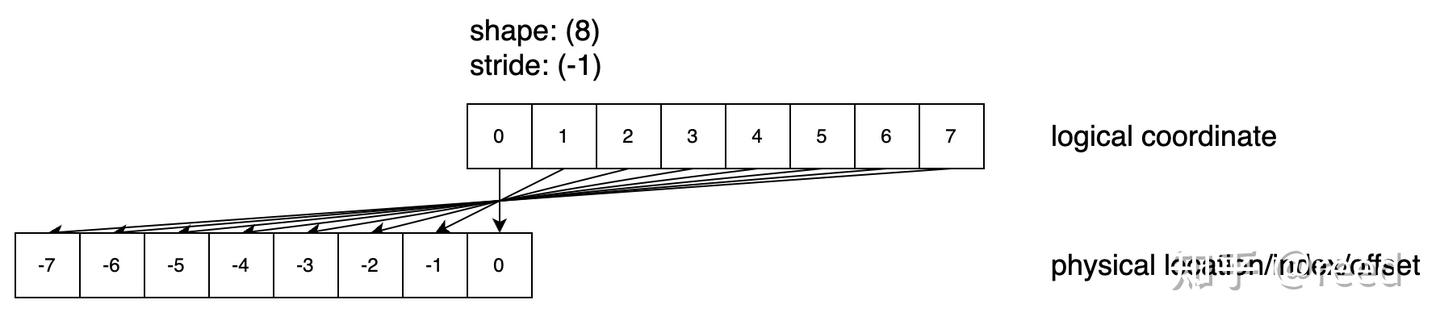
\includegraphics[width=0.9\textwidth]{figures/reed-01-layout/fig-04.jpg}
\end{figure}

Figure 4. shape = 8, stride = -1的逻辑空间和物理空间的映射关系

以上一维空间的示例，呈现了Tensor在其shape不变的情况下，通过stride的改变可以描述tensor中的各个元素在物理空间中的位置。我们在使用Tensor时候，关注的是其逻辑的大小，而通过stride则将这个逻辑空间和实际存储的物理空间进行了关联。并且在计算层面，我们可以看到其始终满足 index = coordinate * stride；

\section{二维矩阵的表示}

Shape: (3, 4), Stride: (1, 3)，和一维向量比较类似，此次的二维空间指的是Tensor的逻辑空间，其存储结构依然可以是一维的，二维空间的列优先描述可以表达为 shape(3, 4), stride(1, 3), 如图5，shape中的3，4分别表示矩阵的行数和列数，stride中的1，3分别表示元素沿着行增加1则物理存储相对的加1，而其中的3则表示如果元素沿着列增加1则其在存储空间的位置需要增加3。

\begin{figure}[htbp]\centering
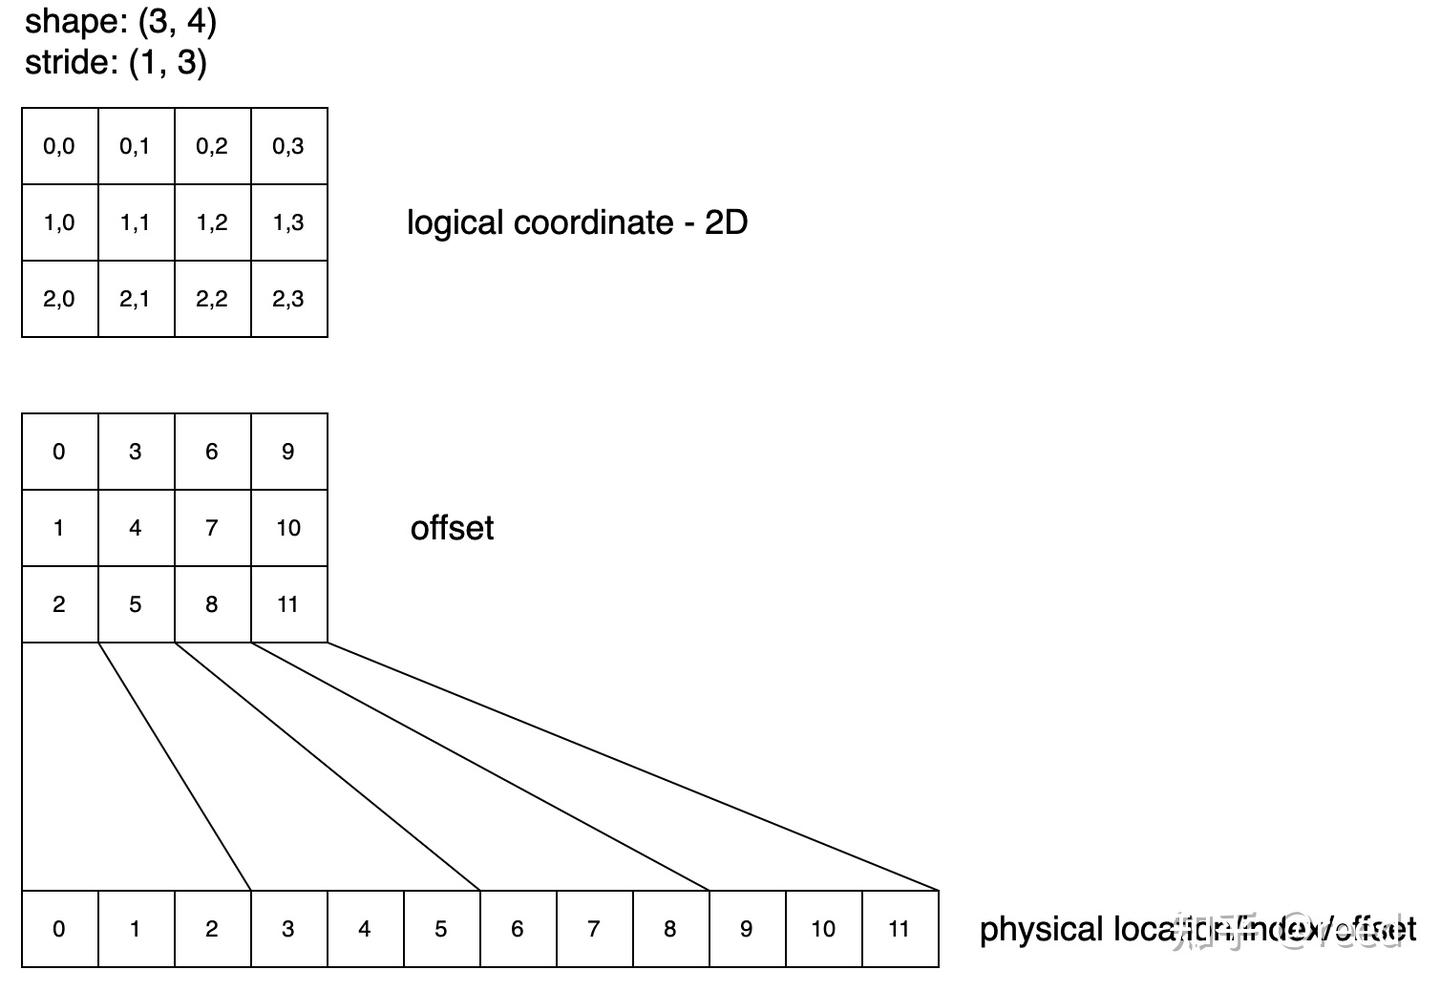
\includegraphics[width=0.9\textwidth]{figures/reed-01-layout/fig-05.jpg}
\end{figure}

Figure 5. shape = (3,4) stride = (1, 3)的逻辑空间和物理空间的映射关系

Shape: (3, 4), Stride: (4, 1)，和上面类似，Shape不变，而stride由(1，3)变为(4, 1)则存储结构变为行优先，即在物理存储数据的时候先存储每一行，行内元素存储的优先级高。

\begin{figure}[htbp]\centering
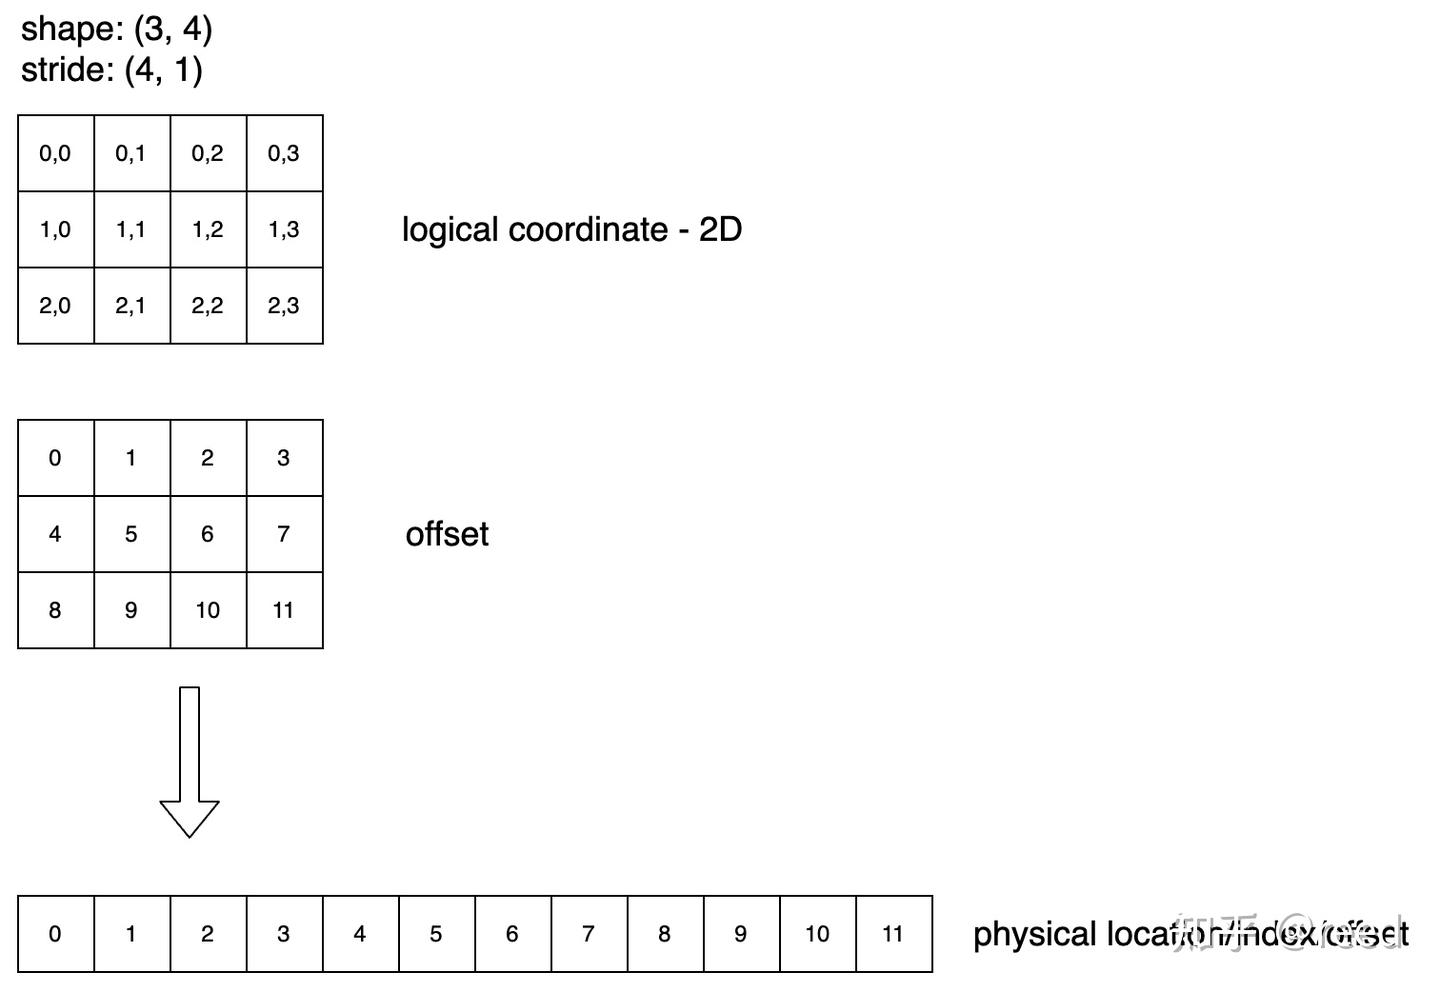
\includegraphics[width=0.9\textwidth]{figures/reed-01-layout/fig-06.jpg}
\end{figure}

Figure 6. shape = (3, 4) stride = (4, 1)的逻辑空间和物理空间的映射关系

二维矩阵的描述和一维类似，shape表示其逻辑形状，stride表示具体的某个元素和物理空间的映射时的间隔量。逻辑空间到物理空间的映射通过点积来完成。从二维空间我们可以很容易的扩展到高维空间，如深度学习常用的（N，H，W， C），其映射关系依然利用点积公式：

\begin{equation*}
index_{physical} = coordinate * stride = \sum_{i}{coordinate_{i} . stride_{i} }
\end{equation*}

\section{有层次的Layout（Heriarchy Layout）}

以上介绍的一维向量和二维矩阵描述描述被深度学习框架所广泛采用，在torch中我们可以访问tensor的shape属性和stride方法（注意方法调用需要使用带括号形式，即stride()）来获取对应的信息。我们不难发现，上面的shape和stride描述其限制了Tensor的每一个轴只能有一个stride值，也就是说，整个tensor在某一个维度上的连续性关系是不能变的，更形象地描述则为：Tensor不可以分块。我们将这样轴的连续性不可变更，体现为Tensor不可以分块的描述称为单调Tensor描述。而当我们处理复杂的Tensor计算问题时，尤其是如NVidia硬件引入的指令计算时，这种表示是不充分的。由此则引入了有层次的Tensor描述，即Heriarchy Layout。简单地理解，有层次的Tensor（或者Layout）就是以原有的单调Tensor所描述的小块作为基础单元，将其组成Tensor。这样原有的小块是Tensor，小块作为单元的外部组织也是Tensor，实现了Tensor套Tensor，这就是所谓的有层级的Tensor了。而其坐标到实际物理位置的映射关系则就是其Layout，Tensor有了层次，Layout也就有层次了。

\begin{figure}[htbp]\centering
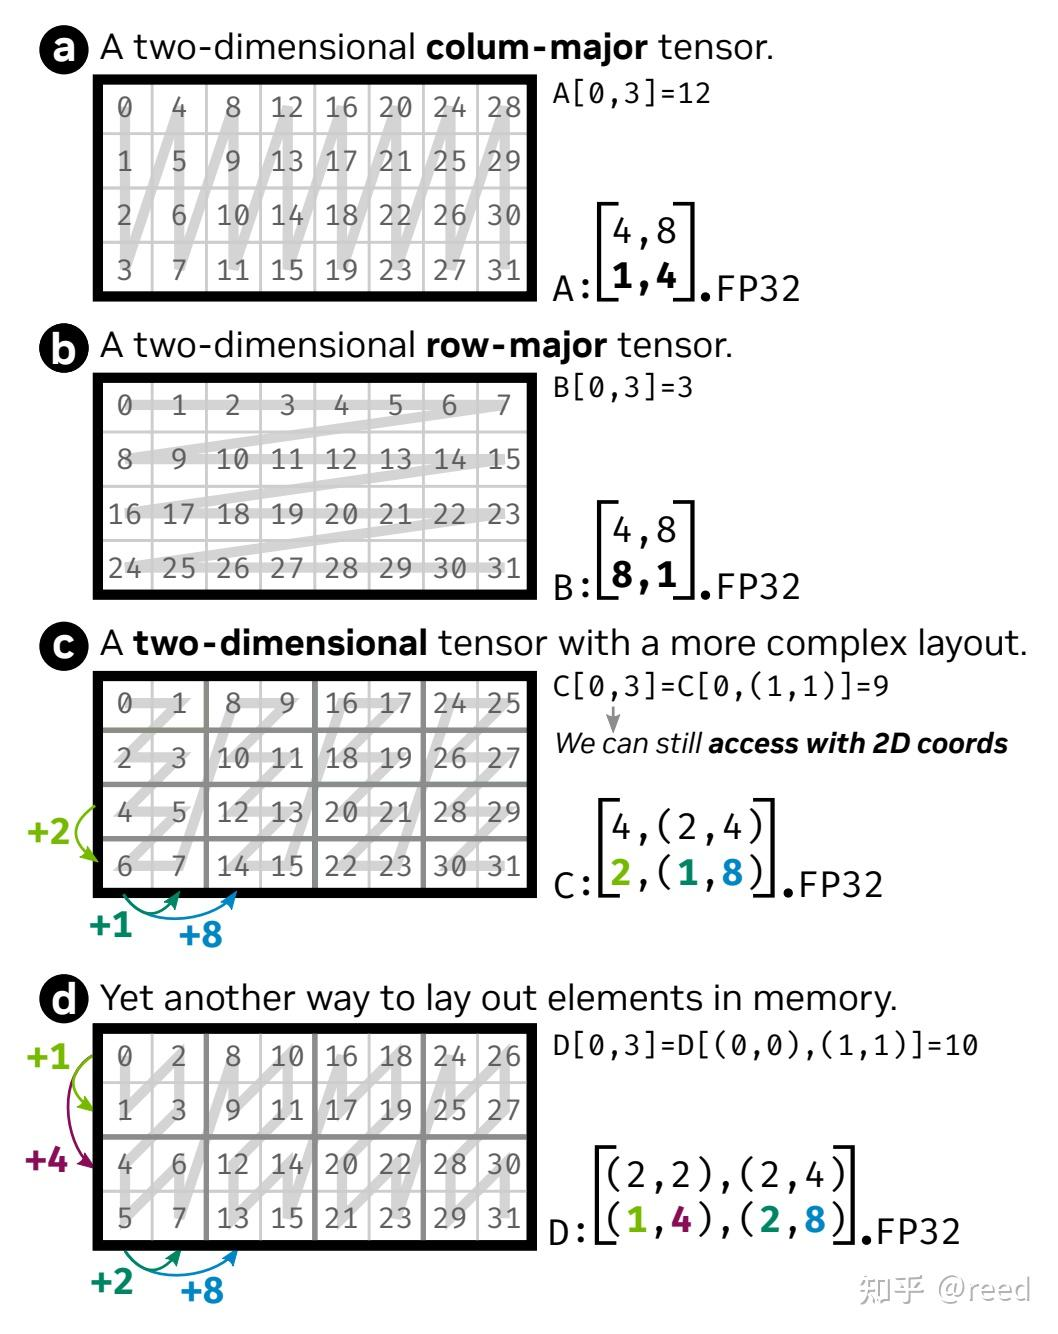
\includegraphics[width=0.9\textwidth]{figures/reed-01-layout/fig-07.jpg}
\end{figure}

Figure 7. 有层次的逻辑空间和其offset计算（引用自ASPLOS23 Graphene IR）

如图7-a/b，它们表示了传统的列优先和行优先的Layout，可以认为它们是一层的Tensor；而图7-c/d用之前的shape和stride描述没有办法表示如此复杂的情况（存在不单调的轴）。此时，我们可以将图7-c图看作两个层级的Tensor，如图8所示，其中内层Tensor为红框所标注的部分，外层Tensor为以红框作为元素的外层Tensor，内层Tensor的shape和stride描述可以表示为shape: (4, 2), stride: (2, 1)，外层Tensor的Layout可以表示为 shape: (1, 4), stride: (4, 1). 两层Tensor合并后，表示整体表示为 4行，8列，其中列方向为两个层次，即 8=2x4列，表示为(2, 4)列，其中2表示内层的Tensor维度为2，4表示列方向上外层Tensor有4个元素。即层级的shape 表示为 （4，(2, 4)）第一个4表示有4行，第二个4表示外层Tensor重复4列，2表示内层Tensor为2列。我们清楚了shape中的各个元素的含义后，stride的形式要与性状保持一致，即stride 要满足 (x, (y, z))的形式，根据x位置对应的含义，表示内层（红框内矩阵）矩阵的行方向的间隔，则有 x = 2；y为内层红框内列方向的间隔，有y = 1；z 则表示红框和红框之间横向的间隔，可以用第二个红框的左上角元素8和第一个红框对应的左上角元素0相减得到，即 z = 8 - 0 = 8, 这样我们得到有层次的Tensor的shape和stride描述：shape: (4, (2, 4)), stride: (2, (1, 8))。

\begin{figure}[htbp]\centering
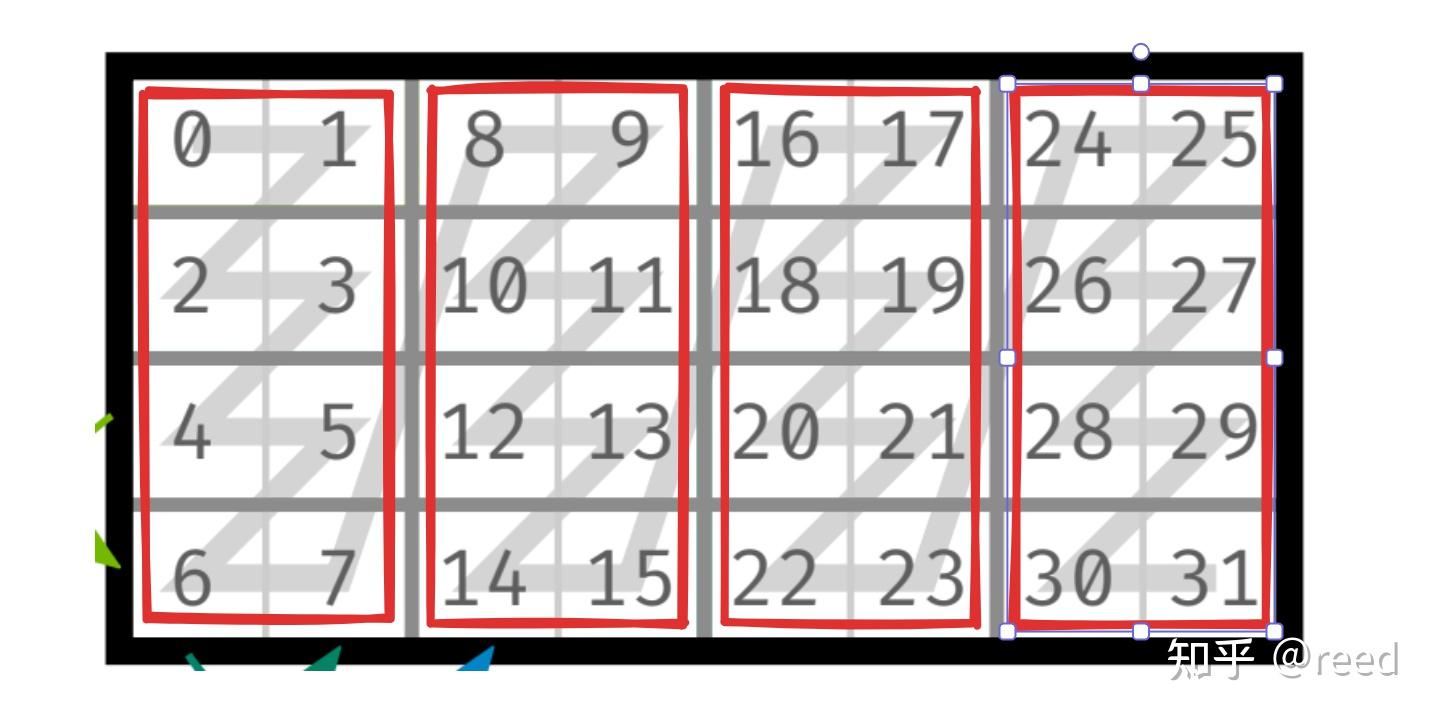
\includegraphics[width=0.9\textwidth]{figures/reed-01-layout/fig-08.jpg}
\end{figure}

Figure 8. 图7-c Tensor的层次分解

图7-d的层次分解和上面类似，其也是两层的结构（如图9）：内层的Tensor为红框所标注，shape: (2, 2), stride: (1, 2)；外层的Tensor为绿线所标注，shape: (2, 4), stride: (1, 2)；合并后的层次化表示 shape: ((2, 2), (2, 4))，其中的数字2，2，2，4分别表示内层Tensor行数，外层Tensor行数，内层Tensor列数，外层Tensor列数。同样的根据以上数据所表示的轴的信息，可以得到 stride: ((1, 4), (2, 8))。

\begin{figure}[htbp]\centering
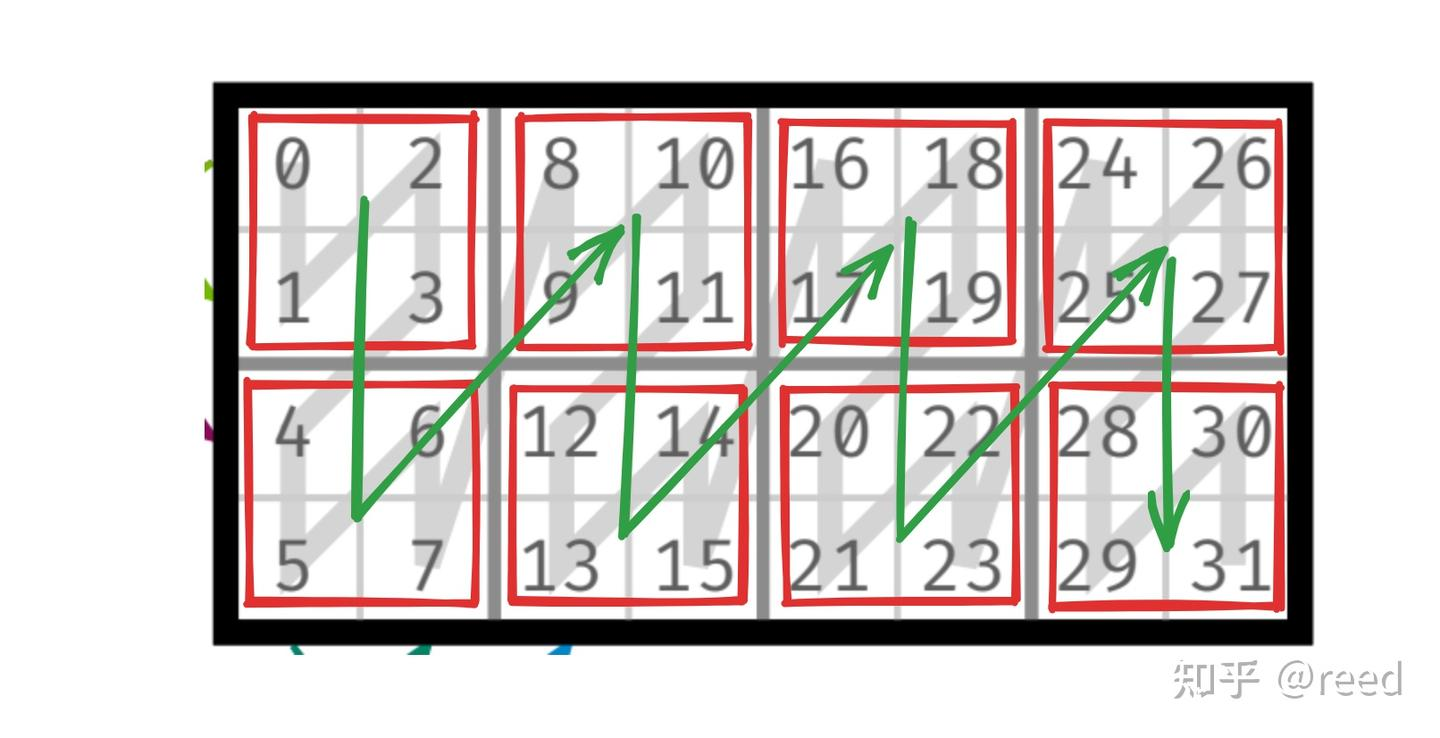
\includegraphics[width=0.9\textwidth]{figures/reed-01-layout/fig-09.jpg}
\end{figure}

Figure 9. 图7-d Tensor的层次分解

shape和stride给出了Tensor的逻辑空间描述和映射到物理空间时的间隔描述，当根据逻辑空间的位置获得物理空间位置时，依然和传统的Tensor计算规则一样，采用coordinate和stride点积即可，只不过坐标也采用heriarchy表达即可。

通过以上两个有层次Tensor的shape和stride的分解和组合，我们可以完成有层次的Tensor的组合，其突破了传统的Tensor轴只能有一个stride的限制，可以表达更丰富的Tensor（有层次的Tensor）。

以上介绍了有层级的Layout描述，具体的在cute实现时，其提供了make\_shape和make\_stride接口，并且make\_shape的参数可以接受make\_shape的结果，以此来完成有层次的shape和stride构建，为了提升效率，shape和stride可以区分为常量shape和变量shape。

\section{常量Shape（编译时Shape）}

常量Shape，即编译时Shape，可以通过在编译时完成坐标的映射或者推导，而减少运行时的计算量。对于需要编译时确定的量，需要用编译时常量来实现，如矩阵分块的大小其依赖了寄存器空间申请则必须使用这种类型shape，其书写形式为Int$<$K$>$\{\}，其中Int表示编译时常量，K表示具体的数值，{}表示以前面的类型来构造一个对象（常量对象），实例如下：

\begin{lstlisting}[language=C++]
auto shape = make_shape(Int<2>{}, Int<3>{});
auto shape1 = make_shape(shape, Int<3>{});
\end{lstlisting}

\section{变量Shape（运行时Shape）}

有些维度信息是运行时决定的，如vector长度等，而且不需要编译时决策，则采用运行时计算模式，值得注意的是示例代码中的2，3虽然是常数，但是在cute的约定里，该形式表示变量。

\begin{lstlisting}[language=C++]
auto shape = make_shape(2, 3);
auto shape = make_shape(m, n);
\end{lstlisting}

\section{总结}

Layout的本质是函数，其可以实现由一种坐标系统变换到一个表示偏移量的标量，超参为Tensor的逻辑shape和stride，即

\begin{equation*}
offset = Layout^{shape}_{stride}(coordinate)
\end{equation*}

\section{参考}

\begin{itemize}
  \item \url{https://dl.acm.org/doi/abs/10.1145/3582016.3582018}
  \item \url{https://github.com/NVIDIA/cutlass/tree/main/media/docs/cute}
\end{itemize}

\section{参考}

\begin{itemize}
  \item \url{https://dl.acm.org/doi/abs/10.1145/3582016.3582018}
\end{itemize}
